\documentclass[11pt,a4paper,english]{article}
\usepackage[T1]{fontenc}
\usepackage[obeyspaces,spaces,hyphens]{url}
\usepackage{amsmath}
\usepackage{amsfonts}
\usepackage{amssymb}
\usepackage{graphicx}
\usepackage{fancyhdr}
\usepackage[left=2cm, right=2cm, top=2cm, bottom=2.00cm, bindingoffset=1.5cm, headheight=1.5cm, includeheadfoot]{geometry}
\usepackage[style=ieee]{biblatex}
\usepackage{xpatch}
\usepackage[english]{babel}
\usepackage{listings}
\usepackage[printonlyused, withpage]{acronym}
\usepackage[hidelinks]{hyperref}
\usepackage{cleveref}
\usepackage[style=german]{csquotes}
\usepackage{siunitx}
\usepackage[onehalfspacing]{setspace}
\usepackage{rotating}
\usepackage{subfig}
\usepackage{multirow}
\usepackage{colortbl}
\usepackage{threeparttablex}
\usepackage{arydshln}
\usepackage{caption}
\usepackage{chngcntr}
\usepackage{float}
\usepackage{tabularx}
\usepackage{pdfpages}
\usepackage{color}
\usepackage{xcolor}
\usepackage{enumitem}
\usepackage{rotating}
\usepackage[toc,page]{appendix}
\usepackage{fontspec}
\usepackage[section, nottoc]{tocbibind}
\usepackage[]{easyReview}
\usepackage{varwidth}
\usepackage{lipsum}
\usepackage{hyphenat}

% Load preamble
% Define warnings for hbox
\hfuzz=5pt

% Program English bibliography strings
\DefineBibliographyStrings{english}{
	andothers   = \mkbibemph{et al\adddot},
	url         = [Online]\adddot\addspace Available under,
	urlseen	= {Accessed on:},
}

% Remove empty braces from Online bibtex entries without date
\xpatchbibdriver{online}
{\printtext[parens]{\usebibmacro{date}}}
{\iffieldundef{year}
	{}
	{\printtext[parens]{\usebibmacro{date}}}}
{}
{\typeout{There was an error patching biblatex-ieee (specifically, ieee.bbx's @online driver)}}

% Add command for captioning equations
\newcounter{equationset}
\newcommand{\equationset}[1]{% \equationset{<caption>}
	\refstepcounter{equationset}% Step counter
	\noindent\makebox[\linewidth]{Equation~\theequationset: #1}}% Print caption

% Arabic section numbering
\renewcommand\thesection{\arabic{section}}

% Enable section numbering to depth 3 (=\subsubsection)
\setcounter{secnumdepth}{3}
\setcounter{tocdepth}{3}
\sffamily

% Enable figure/table/equation numbering per section
\counterwithin{figure}{section}
\counterwithin{table}{section}
\counterwithin{equation}{section}

% Set headers for titlepage
\fancypagestyle{titlepage}{
	\fancyhf{}
	\renewcommand{\headrulewidth}{0pt}
	\renewcommand{\footrulewidth}{0pt}
	\fancyhead[L]{
\includegraphics[width=0.6\linewidth]{assets/thm-logo}}
}

% Set headers for contents
\fancypagestyle{thesishead}{
	\fancyhf{}
	\fancyhead[L]{\leftmark}
	\fancyhead[R]{\thepage}
	\fancyfoot[C]{\thepage}
}

% Set style for basic listings
\definecolor{solarized@base03}{HTML}{002B36}
\definecolor{solarized@base02}{HTML}{073642}
\definecolor{solarized@base01}{HTML}{586e75}
\definecolor{solarized@base00}{HTML}{657b83}
\definecolor{solarized@base0}{HTML}{839496}
\definecolor{solarized@base1}{HTML}{93a1a1}
\definecolor{solarized@base2}{HTML}{EEE8D5}
\definecolor{solarized@base3}{HTML}{FDF6E3}
\definecolor{solarized@yellow}{HTML}{B58900}
\definecolor{solarized@orange}{HTML}{CB4B16}
\definecolor{solarized@red}{HTML}{DC322F}
\definecolor{solarized@magenta}{HTML}{D33682}
\definecolor{solarized@violet}{HTML}{6C71C4}
\definecolor{solarized@blue}{HTML}{268BD2}
\definecolor{solarized@cyan}{HTML}{2AA198}
\definecolor{solarized@green}{HTML}{859900}

\setmonofont{Hack}[
Extension        = .ttf, 
Path                  = /usr/share/fonts/TTF/,
UprightFont    = *-Regular,
ItalicFont         = *-Italic,
BoldFont          = *-Bold,
BoldItalicFont  = *-BoldItalic,
Scale                  = 0.8,] 

\setsansfont{NotoSans}[
Extension        = .ttf,
Path                  = /usr/share/fonts/noto/,
UprightFont    = *-Regular,
ItalicFont         = *-Italic,
BoldFont          = *-Bold,
BoldItalicFont  = *-BoldItalic,
Scale                  = 0.8,]

\lstset{
	basicstyle=\footnotesize\ttfamily,
	numbers=left,
	numberstyle=\tiny,
	numbersep=5pt,
	tabsize=2,
	extendedchars=true,
	breaklines=true,
	keywordstyle=\color{red},
	frame=b,
	stringstyle=\color{white}\ttfamily,
	showspaces=false,
	showtabs=false,
	xleftmargin=17pt,
	framexleftmargin=17pt,
	framexrightmargin=5pt,
	framexbottommargin=4pt,
	%backgroundcolor=\color{lightgray},
	showstringspaces=false,
	numberstyle=\color{solarized@green},
	keywordstyle=\color{solarized@magenta},
	stringstyle=\color{solarized@cyan}\ttfamily,
	identifierstyle=\color{solarized@blue},
	commentstyle=\color{solarized@violet},
	emphstyle=\color{solarized@red},
	rulecolor=\color{solarized@base2},
	rulesepcolor=\color{solarized@base2}
}

%Load listings langauges
\lstloadlanguages{
	python
}


%Modify listings captions
\usepackage{caption}
\DeclareCaptionFont{white}{\color{white}}
\DeclareCaptionFormat{listing}{\colorbox[cmyk]{0.43, 0.35, 0.35,0.01}{\parbox{\textwidth}{\hspace{15pt}#1#2#3}}}
\captionsetup[lstlisting]{format=listing,labelfont=white,textfont=white, singlelinecheck=false, margin=0pt, font={bf,footnotesize}}

% Disable auto indenting after paragraph
\setlength\parindent{0pt}

% Set correct names for appendix package
\renewcommand{\appendixname}{Appendix}
\renewcommand{\appendixtocname}{Appendix}
\renewcommand{\appendixpagename}{Appendix}

% Configure locale for siunit
\sisetup{locale=DE}

% Configure bit unit to always be uppercase
\DeclareSIUnit[]{\bit}{Bit}

% Meta information
\author{IIOT Group 4}
\date{TBD} %TODO: adjust the date
\title{Power Consumption Analysis}

% Load bibliography data
\addbibresource{sources.bib}

% Begin main document
\begin{document}

% Disable page numbering
\pagenumbering{gobble}

% Produce titlepage
\thispagestyle{titlepage}

	\begin{center}
		\vspace{1cm}
		{\LARGE Interdisciplinary IoT Project}\\
		\vspace{2cm}
		{\huge\bfseries Power Consumption Analysis}\\
		\vspace{2cm}
		\begin{varwidth}{\linewidth}
			\begin{tabbing}
				Mary Sutharshini Thevathas \= TBD\kill
				Mary Sutharshini Thevathas \> TBD\\
				Axit Kakadiya \> TBD\\
				Brieuc Pesne \> TBD\\
				Devraj Solanki \> TBD\\
				Robin Dietzel \> 5277715\\
			\end{tabbing}
		\end{varwidth}
		
		\vspace{1cm}
		DATE: tbd\\%TODO: set date correctly
		\vfill
		Department of Informationstechnik, Elektrotechnik und Mechatronik (IEM)\\
		Campus Friedberg\\
		\vspace{1cm}
		Specialization: None/interdisciplinary
	\end{center}

	\vspace{3cm}
	
	\begin{tabularx}{\linewidth}{ll}
		Supervisor: & Prof. Dr.-Ing. Fabian Mink
	\end{tabularx}
	
	%\newpage	
	\pagestyle{plain}
	
	\newpage
	\section*{Statement of authorship}
		I hereby declare that I have written this report independently and exclusively using the sources and aids provided.	Contents of this thesis that were taken verbatim or analogously from other sources are marked as such. The report or parts thereof have not been submitted in this or a comparable form to any other examination body and have not been published.\\
	
	\vfill
	\noindent \makebox[7cm][c]{{\Large \color{blue} Büdingen, den 07.06.2023}} \hfill \makebox[7cm][c]{
\includegraphics[width=5cm]{assets/signatures/robin_dietzel}}\par
	\noindent\rule{7cm}{.4pt}\hfill\rule{7cm}{.4pt}\par
	\noindent Place, Date\hfill Signature\par
	\vspace{0.5cm}
	\noindent \makebox[7cm][c]{{\Large \color{blue} Büdingen, den 07.06.2023}} \hfill \makebox[7cm][c]{
\includegraphics[width=5cm]{assets/signatures/robin_dietzel}}\par
	\noindent\rule{7cm}{.4pt}\hfill\rule{7cm}{.4pt}\par
	\noindent Place, Date\hfill Signature\par
	\vspace{0.5cm}
	\noindent \makebox[7cm][c]{{\Large \color{blue} Büdingen, den 07.06.2023}} \hfill \makebox[7cm][c]{
\includegraphics[width=5cm]{assets/signatures/robin_dietzel}}\par
	\noindent\rule{7cm}{.4pt}\hfill\rule{7cm}{.4pt}\par
	\noindent Place, Date\hfill Signature\par
	\vspace{0.5cm}
	\noindent \makebox[7cm][c]{{\Large \color{blue} Büdingen, den 07.06.2023}} \hfill \makebox[7cm][c]{
\includegraphics[width=5cm]{assets/signatures/robin_dietzel}}\par
	\noindent\rule{7cm}{.4pt}\hfill\rule{7cm}{.4pt}\par
	\noindent Place, Date\hfill Signature\par
	\vspace{0.5cm}
	\noindent \makebox[7cm][c]{{\Large \color{blue} Büdingen, den 07.06.2023}} \hfill \makebox[7cm][c]{
\includegraphics[width=5cm]{assets/signatures/robin_dietzel}}\par
	\noindent\rule{7cm}{.4pt}\hfill\rule{7cm}{.4pt}\par
	\noindent Place, Date\hfill Signature\par
	\newpage
	
	% Enable roman page numbering
	\pagenumbering{Roman}

	% tocs
	\newpage
	\tableofcontents
	
	\newpage
	\listoffigures
	
	\newpage
	\listoftables
	
	% table of acronyms
	\newpage
	\section*{Table of acronyms}
	\begin{acronym}
	\addcontentsline{toc}{section}{Index of abbreviations}
	\itemsep=-2em
	\acro{MQTT}{MQ Telemetry Transport}
	\acro{USB}{Universal Serial Bus}
	\acro{UART}{Universal Asynchronous Receiver Transceiver}
	\acro{IC}{Integrated Curcuit}
	\acro{OTA}{Over The Air}
\end{acronym}
	
	\newpage
	
	% Set headers page style with page number in footer as well
	\fancypagestyle{headings}{%
		\cfoot{\thepage}
	}
	\pagestyle{thesishead}
	
	\pagenumbering{arabic}
	
	
	\newpage
	\section{Introduction [MS]}
	Power consumption analysis has playing an important role in the technological advancement world.
	It’s being adapted by various sectors to utilize the energy consumptions and aiming to have an
	understanding of the energy usage patterns. This report implements a methodology to visualize the
	parameters influencing power usage, which are retrieved from the power analyzer.\\
	
	This report aims to analyze the power consumption patterns in the University building in real-time
	based. Data will be collected through several modules and monitoring systems, allowing for a
	comprehensive visualization of power consumption trends.\\
	
	The Power measurements data such as voltages, current, Phase angles are retrieved from the DEIF
	MIC-2 MKII multi-instrument by using Modbus communication protocol and RS485 serial
	communication facilities. Then the data continuously injected to the cloud platform with the help of
	ESP32 microcontroller device. With the help of MQTT protocol, the injected data in the cloud
	subscribed and visualized in grafana in real time basis.\\
	
\section{Objective of the project}
	
	\begin{itemize}
		\item Retrieve the power usage information from DEIF MIC-2 MKII module
		\item Publish the data to the cloud
		\item Subscribe the published data
		\item Graphical visualization of the data in grafana
	\end{itemize}

	\newpage
	\section{Basics}

	\subsection{RS-485 [AK]}
		RS-485 was created by the Telecommunications Industry Association and Electronic Industries Alliance (TIA/EIA) to overcome the disadvantages of the RS-232 serial communication device. It is used in two-wire data transfer.  Via RS-485 serial communication protocol, the master can communicate up to 32 devices via a wire bus connection as shown in the diagram
	
		\footnotetext{ Figure 1 source: https://www.advantech.com/en/resources/white-papers/02cb2f4e-4fb2-4a87-be3b-508325bd61d6}
		\begin{figure}[H]
			\centering
			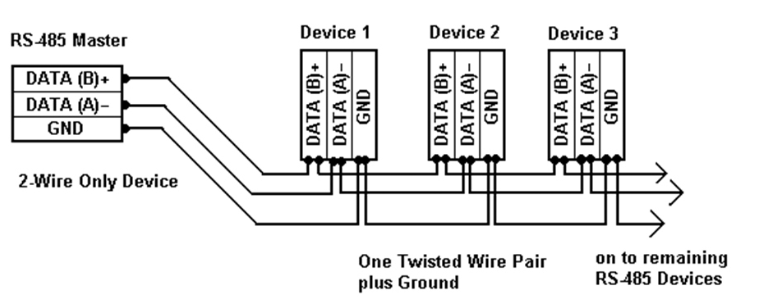
\includegraphics{assets/AK-rs485-masterslave.png}
			\caption{RS-485 Master Slave Connection}
			\label{fig:modbus-master-slave}
		\end{figure}
	
	
		The frame structure of RS-485 is mentioned in the below image. Data transfer will start from High to low pulse (Mark) and then followed by 8 bits of data and then as per the configuration it will use odd parity or even parity. At last low to high pulse (Space) for ending the data transmission.
	
		\begin{figure}[H]
			\centering
			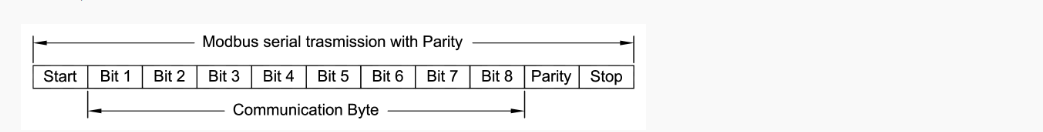
\includegraphics{assets/AK-data-frame-transmission.png}
			\caption{Data Frame Structure Transmission}
		\end{figure}
	
		\footnotetext{ Figure 2 source: https://web-plc.com/blog/2017/06/01/rtu-modbus}
		
		\subsection{Modbus data-link layer [BP]}
		\label{sec:modbus-data-link-layer}
		The following section of this report describes how the Modbus data-link layer works. Modbus works on the data-link layer to trade frames between two device, in the previous part we focused on the electrical part here we will focus on the concept on frames exchange and on frames. 
			
			\subsubsection{The protocol}
				
				\begin{figure}[H]
					\centering
					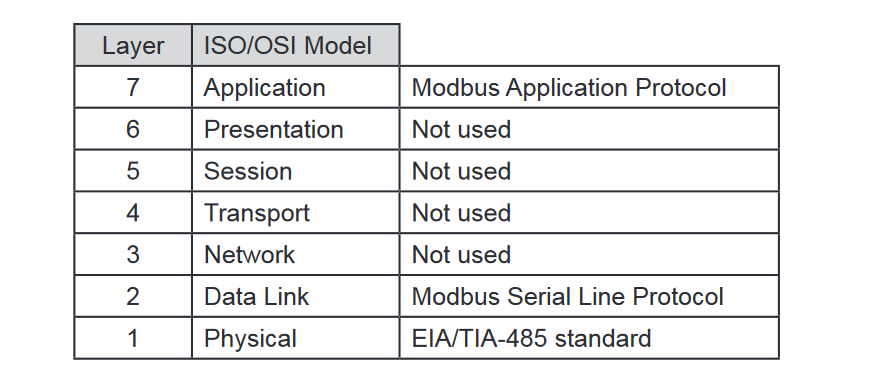
\includegraphics[width=0.7\linewidth]{assets/data-link-layer.png}\qquad
					\caption{Layer where Modbus works~\cite{Modbus-protocol}}
						
					\label{fig:modbus-data-link}
				\end{figure}
			
				The Modbus protocol works on the layer 1, 2 and 7, so there is no interaction between the frame which is sent by the device and how the frame is recieved on the application, that's why it's important to know how this protocol works.
			
				\begin{figure}[H]
					\centering
					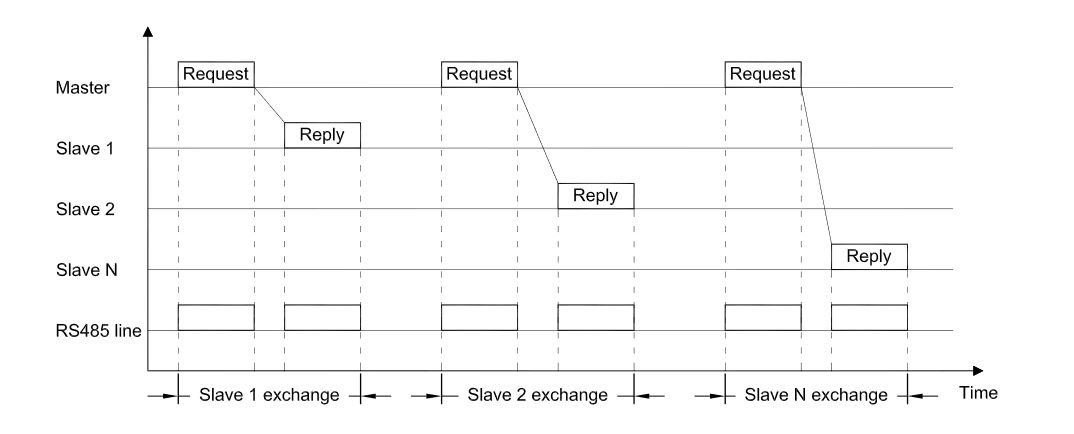
\includegraphics[width=0.9\linewidth]{assets/master-slave-communication.png}\qquad
					\caption{Master slave communication~\cite{Modbus-protocol}} 
					\label{fig:modbus-master-slave-comm}
				\end{figure}
				
				Modbus is based on a master slave communication, the device is consider as the master and send requests to the sensor which is consider as a slave and answer to the request. Each sensor can send informations to multiple device and device can ask different sensors. 
				
			\subsubsection{The frame}
			
				\begin{figure}[H]
					\subfloat[The frame in bytes]{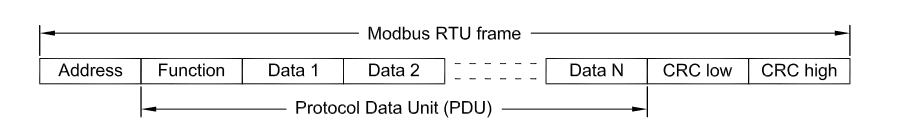
\includegraphics[width=0.5\linewidth]{assets/frame-in-bytes.png}}\qquad
					\subfloat[The frame time]{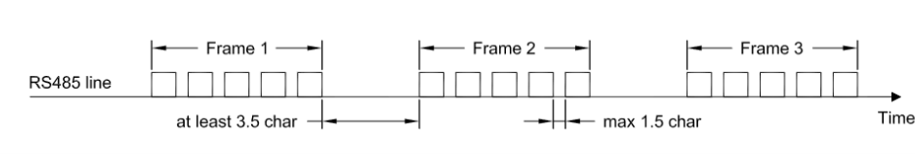
\includegraphics[width=0.5\linewidth]{assets/frame-time.png}}
					\caption{Typical frame~\cite{Modbus-protocol}}
					\label{fig:hw-components}
				\end{figure}
				
				Each frame consists of one byte of addressing to connect to the sensor, one byte of protocol type, as many bytes as necessary for data transfer and two bytes of error control that are important to ensure the integration of communication. Frames are sent in regular time intervals to ensure the integrity of the link (if a delay appears is that a frame is missing).
				
				Traditionally, sensor addresses are~\cite{Modbus-protocol}:
				\begin{itemize}
					\item 0 broadcast for slave
					\item 1 – 247 unicast
					\item 248 – 255 impossible (reserved for the manufacturer)
				
				\end{itemize}
				
				In details, there are two types of bytes, one with a parity cock and one without, this does not change much because it is just replaced by a stop bit.
				
				\begin{figure}[H]
					\subfloat[A byte with parity]{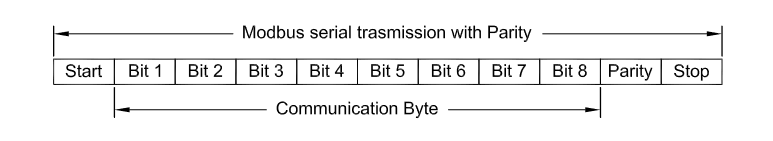
\includegraphics[width=0.5\linewidth]{assets/byte-parity.png}}\qquad
					\subfloat[A byte without parity]{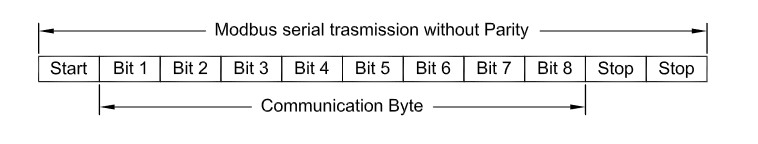
\includegraphics[width=0.5\linewidth]{assets/byte-without-parity.png}}
					\caption{The byte in details~\cite{Modbus-protocol}}
					\label{fig:byte-parity5}
				\end{figure}
		
	\subsection{ESP32 [DS]}
		\label{sec:esp32}
		
		The ESP32 microcontroller family, developed by Espressif System, is very famous for providing best features which are perfectly suited wild range of IoT projects and application. There are many different microcontroller are offered by Espressif, However for this project, ESP32 family’s Microcontroller are well suited as its key features are a dual-core Xtensa LX6 processor, integrated Wi-Fi and Bluetooth capabilities, a robust set of peripherals, and scalable memory options. Here, we've chosen the ESP 32-WROOM 32E microcontroller, embedded in the ESP32 Olimex board,  from the ESP32 family.
		
		\subsubsection{ESP32 WROOM 32 E}
			Since we wish to access our data via a MQTT broker, a variety of connectivity options are important considerations when selecting a device. Here, we've chosen the ESP 32-WROOM 32E micro controller(Depicted on the left side) on the  from the ESP32 family. This has an Ethernet connector, WiFi, and Bluetooth chip built right in.We decided on this ESP32-WROOM 32E rather than an Arduino since an Arduino requires the inclusion of wifi and bluetooth modules. It also has more integrated components, such as an antenna and flash memory, and is quite affordable. These points all satisfy our requirements and are most appropriate for our project.
		
			\begin{figure}[H]
				\centering
				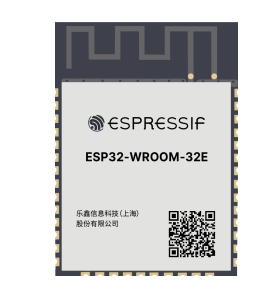
\includegraphics[width=0.4\linewidth]{assets/DS-esp32.png} 
				\caption{ESP32 WROOM 32E processor~\cite{esp-32-package}.}
			\end{figure}
		
		\subsubsection{Dual Core- Processor}
			The module is chipped with dual-core Xtensa LX6 processor, this configuration gives ESP32 to work on different task at a same time with correct output on two processing units. Dual core feature provide upgraded overall performance and multitasking capability. It has clock frequency range from 80 MHz to 240 MHz. This clock frequency is editable by the operator. 
		
		\subsubsection{Pin Configuration}
			\begin{figure}[H]
				\centering
				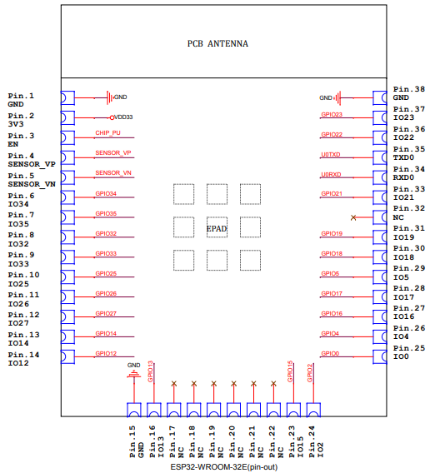
\includegraphics[width=0.4\linewidth]{assets/DS-esp32-pin.png} 
				\caption{Pin configuration~\cite{esp-32-package}.}
			\end{figure}
			This module has a diverse pin configuration. Its has 40 GPIO(General Purpose Input Output) pins(e.g., GPIO04, GPIO12), which gives versatile Analog and Digital communication feature. Furthermore, it also has UART pins (TX0,RX0), by which the serial communication (e.g., RS485 modbus) become very easy. It also have ADC pins, PWM pins, boot and Reset pins, I2C pins and SPI pins.
		
		
		\subsubsection{Wireless Connectivity}
			This processor has inbuilt Wi-Fi(802.11b/g/n), which can operate as station mode and access point mode. Also, it support WiFi communication security with WPA/WPA2. During transmission of data, it can do encryption in order to ensure data security. With WiFi it also have inbuilt Bluetooth support. 
		
		\subsubsection{Memory Configuration}
			The ESP32 WROOM 32E is devided into two different memory type, SRAM \& Flash memory. SRAM(Static Random-Access Memory) it used for storing temporary data, high speed and inorder to improve overall performance of module. On the other hand, Flash Memory is Non-volatile type of memory, where the real program code, firmware and data are stored.
		
	\subsection{ESPHome Introduction [AK]}
		Several options were available for flashing the ESP-32 device like Arduino-IDE, ESP-Home, Platform-IO, etc. To decide which platform, you require you need to consider your application like what purpose you want to solve. Our application was to connect with Text sensors like MQTT subscribers, Modbus, and many more, and ESPHome can do that. Also, ESPHome has an advantage in that it is a web-based interface so you can connect to any device without actually installing that application.
	
		\begin{figure}[H]
			\centering
			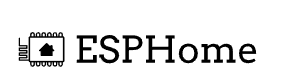
\includegraphics{assets/AK-esphome.png}
			\caption{ESPHome Firmware Logo}
			\label{fig:example}
		\end{figure}
	
		\footnotetext{ Figure 1 source: https://esphome.io}
	
		\setlength{\parindent}{0pt}
	
		ESPHome uses YAML (Yet Another Markup Language) for configuration, making it accessible to users without extensive programming experience. We can start with the ESPHome in several ways, like Using a Command line, From the Home assistant, and using a Docker container. Due to ESPHome’s inherent Modbus compatibility, you can link to any Modbus network and interact with any Modbus-compatible sensor. One of ESPHome's major benefits over other firmware devices is that it is an open-source platform with a vibrant and expanding community of users. If you run into any issues, you can always reach out to the community for help. Furthermore, over-the-air upgrades are supported by ESPHome, enabling users to access the device virtually.
		
	\subsection{MQTT [MS]}
		Message Queuing Telemetry Transport (MQTT) is open-source, lightweight, and publish-subscribe
		messaging protocol. Primarily designed for the communication among the devices those contain the
		resource.
		
		\subsubsection*{Features}
			\begin{description}
				\item[Publish-Subscribe-Architecture]  It uses publish-subscribe model, which allows the devices to act as
				publishers or subscribers.
				\item[Broker-Based Communication]  MQTT communication relies on a broker that acts as a mediator
				between publishers and subscribers. The broker efficiently manages message routing to ensure
				messages reach the intended recipients.
				\item[Topics]  Communication in MQTT uses topics, hierarchical strings used to categorize messages.
				Subscribers express interest in specific topics, and publishers send messages to these topics.
				\item[\acf{QoS} Levels] MQTT provides configurable levels of reliability (QoS Levels 0, 1,
				2)
				\item[Security Features] Transport Layer Security (TLS) encryption, can be implemented to secure MQTT
				communication.
				\item[Retained messages] the broker stores a last known good value for new subscribers
				\item[Persistent sessions] the broker stores messages on behalf of a subscriber that is temporarily offline
				\item[Heartbeats]  if the broker does not receive a PINGREQ for some time, it will close the connection and
				send the Last Will and Testament (LWT)
				\item[\acf{LWT}] A predefined message sent to all subscribers by the broker in case a
				device stops responding.
			\end{description}
	
	\subsection{DEIF MIC-2 MKII [MS]}
		DEIF MIC-2 MKII is a multi-instrument used to monitor and control the operations. The unit
		continuously updates metering results and allows users online access to monitor. It has the
		capability of logging from single low voltage to multiple high voltage parameters. All
		metering data and setting parameters can be accessed by using the front panel keys or with the
		communication port. Setting parameters are stored in the EEPROM.
		
		\begin{figure}[H]
			\centering
			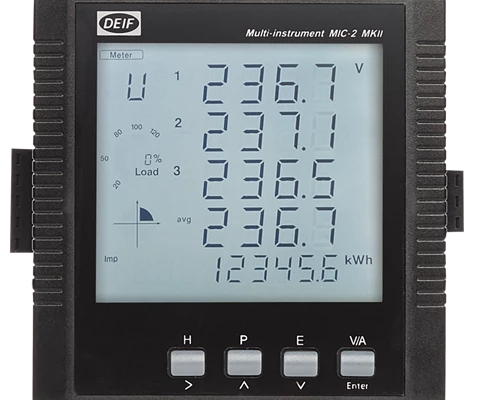
\includegraphics[width=0.6\linewidth]{assets/MS-deif.png}
			\caption{DEIF MIC 2 MKII~\cite{deif-mk2}}
			\label{fig:deif-mic-mk2}
		\end{figure}
		
		\subsubsection*{Features}
			\begin{itemize}
				\item Multiple connected devices- Uses RS-485 Modbus communication (Up to 32 devices
				can be connected on a RS485 bus)
				\item Customized alarm settings- facilitate to customize upto16 different parameters
				\item Password protected setting- Counter reset and change of settings can be password-
				protected
				\item Display- Large LCD screen with white backlight
				\item Control and Monitoring- It provides a user interface for operators to monitor the
				parameters and control its operation.
				\item Communication- the instrument support various communication modules - Ethernet
				(Modbus TCP, HTTP, SMTP), Profibus DP
				\item Remote Access- Remote monitoring and control capabilities allow users to access and
				manage the generator set from a distance.
				\item Inputs and Outputs- Optional Input and Output modules - Relay , Analogue I/O,
				Digital I/O
				\item Data Logging-It may include data logging features, allowing operators to analyze
				historical performance data and identify trends.
				\item Customizable Configurations- Users may have the ability to configure the controller to
				meet specific application requirements, adapting it to different measurements and
				operational scenarios.
			\end{itemize}
	
	

	
	\newpage
	\section{Main-part} %TODO: rename properly
	\subsection{Hardware suggestion}
\label{sec:hardware-suggestion}
	The following section of this report describes the hardware and software suggestion for interfacing with the \texttt{MIC-2 MKII's} modbus interface. The hardware/software stack should be able to readout several registers of the device over modbus. Then the data should be sent via \ac{MQTT} to a broker within the THM network for further processing and visualization.

	\subsubsection{Development board}
		As the microcontroller development-board was picked the \texttt{OLIMEX ESP32-GATEWAY} board. Olimex is a provider of development boards, embedded device programmers and other development tools.~\cite{olimex}
		The board itself is depicted within \cref{subfig:hw-components} on the left side. The following list gives a brief overview about the features of this development board.
		\setlist{noitemsep}
		\begin{itemize}
			\item ESP32-WROOM32 module
			\item CH340B USB-UART converter for programming
			\item Ethernet 100MB interface (LANA710A phy chip)
			\item MicroSD card slot
			\item 20-Pin GPIO connector with all ESP32 ports
		\end{itemize}
		\begin{figure}[H]
			\subfloat[OLIMEX ESP32-GATEWAY]{\includegraphics[width=0.5\linewidth]{assets/RD-esp32-gateway.png}}\qquad
			\subfloat[RS485 module~\cite{IMG-rs485conv}]{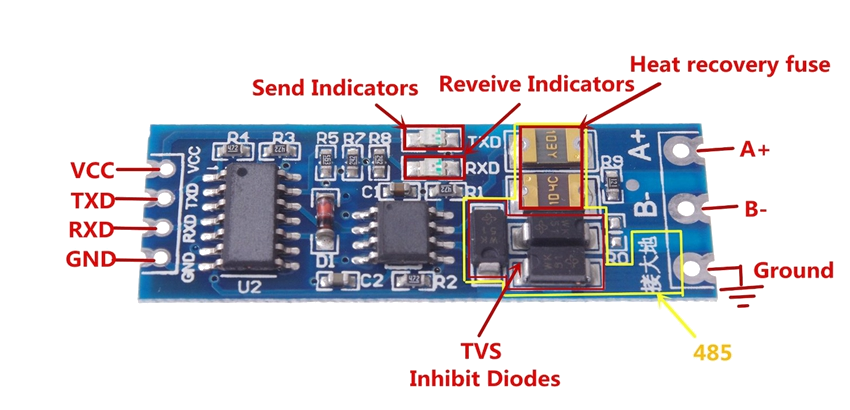
\includegraphics[width=0.5\linewidth]{assets/RD-rs485-converter.png}}
			\caption{Selected hardware for connection with \texttt{MIC-2 MKII}}
			\label{subfig:hw-components}
		\end{figure}
			The board seems to be well suited for this application because it's quite cheap with an average price of $ 16.59 € $ (in 11/01/2023) and has an onboard ethernet transceiver and port. The ethernet port was one of the main criteria when picking the board because wireless communication form inside the wiring closet, where the device should be placed, might not be a good choice for reliable communication. The onboard \texttt{CH340B} chip brings the advantage to easyly flash the board without an externel \ac{USB} to \ac{UART} converter. This gives more flexiblity when developing the firware for the board. The onboard sdcard is not really necessary in the context of this work.\\ %TODO: ggf beschreiben dass man werdte puffern kann
			At least there is one other advantage to mention here: The board has open-source hardware, so the schematics can be freely browsed in the internet.
	\subsubsection{RS485 interface}
		The pickd RS485 interface is depicted in \cref{subfig:hw-components} on the right hand. The module then connects to the development board with $ 3.3~\si{\volt} $ supply voltage and ground. The \texttt{TXD} and \texttt{RXD} pins connect the \ac{UART} interface between the board and the converter. On the right edge of the converter module you can see the \texttt{A+} and \texttt{B-} pins which later will be connected to the modbus device. They communicate over RS485 levels. Unfortunately the chip on the converter was milled of so that it was impossible to lookup the \ac{IC} used on those types of boards.
		
		\begin{figure}[H]
			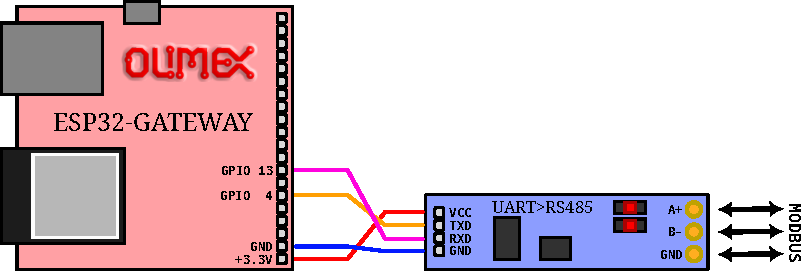
\includegraphics[width=\linewidth]{assets/RD-esp-rs485-hw-conn.pdf}
			\caption{Schematic of connection between ESP32-GATEWAY board and the RS485 converter}
			\label{fig:gw-converter-hwconn}
		\end{figure}
		
		The precedent \cref{fig:gw-converter-hwconn} outlines the wired connections between the UART to RS485 converter used in this project with the ESP32-GATEWAY board. For mounting and installing those two connected boards in the wiring cabinet it will aditionally be necessary to design an enclosure. This will be further described in TBD.%TODO: cref auf kapitel mit 3d gehäuse!
		The GPIO-Pins $ 4 $ and $ 13 $ were chosen because they aren't occupied by specific hardware functions already present on the development board (e.g. SD-Card slot). One additional challange was not to use pin $ 12 $ because it's a \enquote{strapping} pin. Those pins must be left floating or pulled to ground when flashing the device.
		
	\subsubsection{Case-design}
		For installing the device a kind of case should designed to avoid short-circuits or other damage to the hardware when placing it somewhere. Therefore a very simple base-plate was desgined and 3D printed in order to protect the bottom of the ESP32-GATEWAY's board.
		
		\begin{figure}
			\centering
			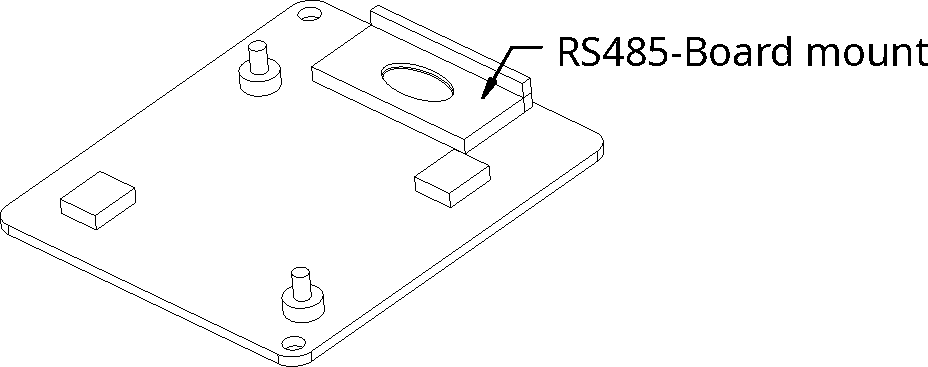
\includegraphics[width=0.8\linewidth]{assets/RD-board-mount}
			\caption{ESP32-GATEWAY + RS485 Converter Board mount}
			\label{fig:board-mount}
		\end{figure}
		
		\Cref{fig:board-mount} shows an exported 3D drawing created with the CAD-Application FreeCAD. The real mount was printed on a Prusa Mini+ 3D printer with PLA filament. After mounting the board the bolts were molten with a soldering iron to hold the board in-place. The RS485 Board was glued onto the mount.
	\subsection{Software suggestion}
\label{sec:software}
%TODO: link section to esphome in first sentence
	This section contains a basic explanation which software/firmware was chosen for operating the ESP32-GATEWAY board described in \cref{sec:hardware-suggestion}. Thus this section contains the basic configuration used to do \ac{OTA} updates and configuration provisioning.\\
	
	For building and installing the esphome firmware, an esphome server must have been set up in a containerized environment. This procedure is described in \cref{sec:esphome-container}.  The following listing contains the basic configuration in the \ac{yaml} format that was used to build the esphome firmware for the device. It configures ota-updates and the basic connection to the \ac{MQTT} server. Some parts of the configuration were left out because they are not relevant in this scope. The second listing provides the configuration for a single modbus register as an example. All other registers were configured in the same scheme. 
	
	\subsubsection{General configuration}
		\begin{lstlisting}[tabsize=2, gobble=4, caption={Basic esphome configuration}, label=lst:esphome-basic]
		esphome:
			name: $dev_name
			friendly_name: $dev_name
		
		esp32:
			board: esp32-gateway
			framework:
				type: esp-idf
		
		ethernet:
			type: LAN8720
			mdc_pin: GPIO23
			mdio_pin: GPIO18
			clk_mode: GPIO17_OUT
			phy_addr: 0
			use_address: $current_ip 
	
		ota:
			password: "82c8244b10a089f5f56db37378ed616c"
		
		web_server:
			port: 80
			auth:
				username: $auth_username
				password: $auth_password

		time:
			- platform: sntp
				id: sntp_time
				timezone: Europe/Berlin
				servers: $ntp_server
		

		text_sensor:
			- platform: ethernet_info
				ip_address:
				name: "IP-Address"
	
		mqtt:
			broker: $mqtt_broker
			port: $mqtt_port
			username: $mqtt_auth_username
			password: $mqtt_auth_password
			client_id: $dev_name
			topic_prefix: "/IoT"
			log_topic: "/system/log"
			keepalive:
				seconds: 5
			skip_cert_cn_check: False
			idf_send_async: False
			certificate_authority: |
		-----BEGIN CERTIFICATE-----
		<PLAINTEXT CERTIFICATE REMOVED FOR BETTER READIBILITY>
		-----END CERTIFICATE-----
		
		
		uart:
			id: modbus_ua
			tx_pin: 4
			rx_pin: 13
			baud_rate: $mb_baudrate
			data_bits: 8
			stop_bits: 1
			parity: NONE
		
		modbus:
			id: modbus0
			uart_id: modbus_ua
			send_wait_time: 250ms
			disable_crc: False
		
		modbus_controller:
			-	id: deif_mic2
				address: $mb_slave
				modbus_id: modbus0
				update_interval: $update_interval
				command_throttle: 0ms
		\end{lstlisting}
	\subsection{Software (Server side)}
	On the server side of this project a flexible and secure approach was picked to deploy several services in an easy manner. To fullfill these conditions we make use of containerization using \texttt{Docker}.\\ Within \texttt{Docker} a container is an isoleted environment for running code. The container has no knowledge of the operating system or the filesystem. A container includes everything needed for the containerized application to run, including all library dependencies and the base operating system~\cite{docker-gstarted}.\\
	The docker daemon\footnote{Managing background process for docker containers} was deployed on a \texttt{Debian 6.1} virtual server provided by the THM. At the beginning of this project only SSH-Access to this server was available. The setup of the \texttt{Docker} daemon and \texttt{Portainer}\footnote{Webinterface for managing a docker installation} was done together with IIOT-Team1 and Professor Mink. The following subsection describes briefly how this was accomplished.
	
	\subsubsection{Docker and Portainer setup}
		The enumeration outlines the basic installation and setup process:
		\begin{enumerate}
			\item Upgrade software on the server to the lates releases
			\item Installation of docker daemon according to the official instructions~\cite{docker-install}
			\item Join ssh-user into docker group (rootless control of Docker daemon)
			\item Deploy the \texttt{Portainer} container
			\item Configure basic Portainer settings\footnote{It's best-practice to disable bind-mounts in portainer so that Portainer users cannot mount and access the root directory within a container}
			\item Create user accounts for team members
		\end{enumerate}
		
		This setup provides options to easily deploy docker containers for all team-members without having ssh access onto the server. Portainer also adds user managment ontop of the Docker daemon. Thus simple accounting rules can be applied on the different users so their usable ressources on the server can be limited. 
		
	\subsubsection{Esphome deployment}
	\label{sec:esphome-container}
		This section explains the deployment of an esphome server used to configure and build the firmware for the hardware described in \cref{sec:hardware-suggestion}. Esphome was deployed using \texttt{docker compose}. Docker compose is a kind of wrapper for the docker command line interface. In general you define a \enquote{stack} in the \ac{yaml} file format where you configure all containers, which ports to expose and which volumes/directories to mount into the container. Such a yaml file was set-up within the portainer webinterface containing the following configuration:
		
		%TODO: fix yaml appearence in listings
		\begin{lstlisting}[tabsize=2, gobble=4, caption={docker-compose.yml configuration for esphome container}, label=lst:esphome]
		esphome:
			image: esphome/esphome
			container_name: esphome
			restart: unless-stopped
			ports:
				- "20000:6052" # Web dashboard
			networks:
				- dev-net
			volumes:
				- team4-esphome_team4_esphome_conf:/config
			environment:
				USERNAME: "admin"
				PASSWORD: "iotlab2023team4"
				ESPHOME_DASHBOARD_USE_PING: true
		volumes:
			team4-esphome_team4_esphome_conf:
			external: true
		\end{lstlisting}
		
		In this configuration file a new container with the name \enquote{esphome} is deployed. The virtual docker volume \enquote{team4-esphome\_team4\_esphome\_conf} is mounted according to the esphome documentation within the container under the path \enquote{/config}. The default esphome port \texttt{6052} is exposed as port \texttt{20000} to not overlap with ports assigned to team 1.\\
		After deploying that container this way the web interface of esphome was available under the given port. From that web interface our team was able to deploy and build the yaml-based configuration for the device and also flash it onto the device via the \ac{OTA} update feature. The configuration itself is explained in detail in \cref{sec:software}. Of special interest is the environment variable \texttt{ESPHOME\_DASHBOARD\_USE\_PING}. This enables the dashboard to discover the esphome device's online status by using ping and not \ac{mDNS}. This configuration change is essential because \ac{mDNS} would not work in the THM network.
		
	\subsubsection{Node-Red Grafana and Influxdb}
	
	\subsubsection{Telegraf}
		Telegraf is a sofware developed by Influxdb and has the main task to scrape data from via different souce plugins and push them into an influxdb instance. This tool is highly integrated with influxdb, thus configuration for a telegraf process cand be directly generated from an influxdb. In the influxdb's web interface you can add a new \enquote{Telegraf} as data source. Then a configuration editor pops up, where the previously deployed \ac{MQTT}-server was configured. The retreived data is published in a single \ac{MQTT} topic in a \ac{JSON} encoded string. Thus the telegraf configuration was set-up so that it parses the \ac{JSON} string and stores all time series data correctly in the influxdb.\\
		The next step consisted of deploying the telegraf instance with docker. \cref{lst:telegraf} shows the configuration. The telegraf agent in the container is started with the environment variable \texttt{INFLUX\_TOKEN} set to the access token provided by the influxdb telegraf integration and the base docker command is appended with the \texttt{--config} option and the url provided by the integration that serves the configuration file. Thus the configuration could be edited dynamically in the influxdb webinterface and the telegraf container re-fetches the configuration on each startup. This way we save ourselves to provide static configuration files for telegraf.
		
		\begin{lstlisting}[tabsize=2, gobble=4, caption={docker-compose.yml configuration for telegraf}, label=lst:telegraf]
		telegraf1:
			image: telegraf
			container_name: telegraf1
			restart: unless-stopped
			networks:
				- dev-net
			environment:
				INFLUX_TOKEN: "boY1r6bdGmwU00Sou-f-VrFuh4zlQovnLbRDaqRQyZNkybBSSg9nwRAlQBL9LlLFr8qNUmdt5dLQAF6IgmouXw=="
			command: "--config http://influxdb:8086/api/v2/telegrafs/0c4903c473f8e000"
		\end{lstlisting}
		
		The configuration for the telegraf agent available under the url in \cref{lst:telegraf} in the last line is summarized in the following listing:
		
		\begin{lstlisting}[tabsize=2, gobble=4, caption={Telegraf configuration}, label=lst:telegraf-cfg]
		[agent]
		interval = "10s"
		round_interval = true		

		[[outputs.influxdb_v2]]
			urls = ["http://mt-labor.iem.thm.de:20002"]
			token = "$INFLUX_TOKEN"
			organization = "iot-team4"
			bucket = "iot-data-telegraf"
		
		[[inputs.mqtt_consumer]]
			servers = ["ssl://emqx:8883"]
		
			topics = [
				"/IoT/combined"
			]
		
			client_id = "telegraf-scraper"
		
			username = "admin"
			password = "iotlab2023team4"
		
			insecure_skip_verify = true
		

			data_format = "json"
			json_time_key = "_ts"
			json_time_format = "unix"		
		\end{lstlisting}
		
		As you can see in \cref{lst:telegraf-cfg} the telegraf agent is configured to write data to the database each $ 10~\si{\second} $ and to round the collected data within this interval. The section \texttt{outputs.influxdb\_v2} configures the connection to the indluxdb running within the docker stack. The section labelled \texttt{inputs.mqtt\_consumer} describes the connection to the \ac{MQTT} broker. It was configured to listen only to the json encoded topic \texttt{/IoT/combined}. \texttt{insecure\_skip\_verify} skips the certificate check\footnote{Telegraf still uses an ssl encrypted connection to the broker. Only the CA check is skipped. This saved a bit work to import the CA certificate into the docker container. For true authenticity this should be made up later.}. Of special interest is the option \texttt{json\_time\_key} that defines a \ac{JSON} key in the object received at the provided topic that holds the timestamp to write to the influxdb. \textbf{By using this option the timestamp is not appended when writing to the influxdb, but rather originate from the hardware interface board itself.}

	\newpage
	\section{Conclusion}
	blah

	% Workaround to break urls in bibliography
	\setcounter{biburllcpenalty}{7000}
	\setcounter{biburlucpenalty}{8000}
	\newpage
	\printbibliography [heading=bibintoc]
	
	% Build appendix
	\pagestyle{plain}
	\newpage
	\begin{appendices}
		%\includepdf[
		%	pages=1,
		%	frame=true,
		%	scale=0.8,
		%	pagecommand={
		%		\phantomsection
		%		\addcontentsline{toc}{subsection}{Legende Logikbausteine}
		%		\label{appendix:logiccomponents}
		%	}
		%]
		%{appendix/legend.pdf}
	\end{appendices}
	
\end{document}